\documentclass[border=2pt,tikz]{standalone}

\usepackage{physics}

\usepackage{amsfonts,amssymb,amsmath}
\usepackage{tikz-cd}
\usepackage{tikz}
\usepackage{mathdots}
\usepackage{yhmath}
\usepackage{cancel}
\usepackage{color}
\usepackage{siunitx}
\usepackage{array}
\usepackage{multirow}
\usepackage{amssymb}
\usepackage{gensymb}
\usepackage{tabularx}


\usetikzlibrary{decorations.pathmorphing}

\begin{document}
% Gradient Info


\tikzset{every picture/.style={line width=0.75pt}} %set default line width to 0.75pt

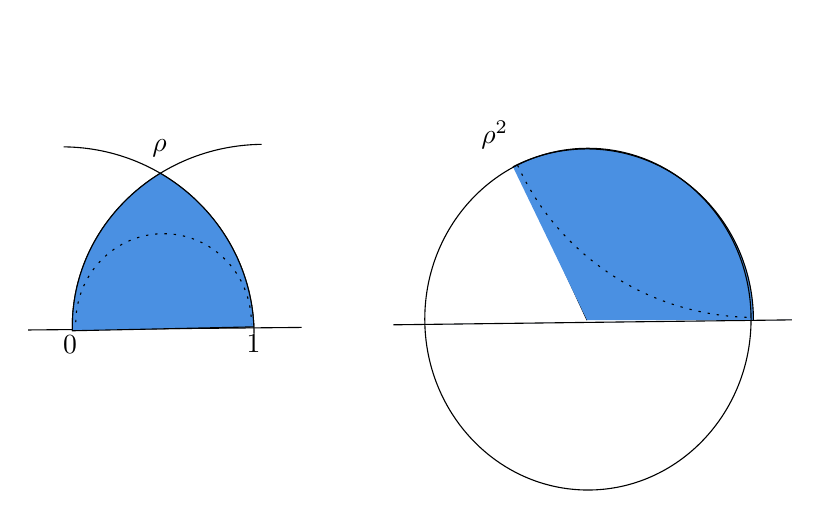
\begin{tikzpicture}[x=0.75pt,y=0.75pt,yscale=-1,xscale=1]
%uncomment if require: \path (0,300); %set diagram left start at 0, and has height of 300

%Straight Lines [id:da922650108701975]
\draw    (43.62,155.43) -- (175.38,154.2) ;
%Shape: Arc [id:dp5359245814939384]
\draw  [draw opacity=0] (60.67,67.21) .. controls (110.98,67.56) and (151.91,107.37) .. (152.42,156.83) .. controls (152.42,156.96) and (152.42,157.09) .. (152.42,157.23) -- (60.05,157.68) -- cycle ; \draw   (60.67,67.21) .. controls (110.98,67.56) and (151.91,107.37) .. (152.42,156.83) .. controls (152.42,156.96) and (152.42,157.09) .. (152.42,157.23) ;
%Shape: Arc [id:dp7932600593552737]
\draw  [draw opacity=0] (64.89,155.86) .. controls (64.88,155.47) and (64.87,155.08) .. (64.87,154.68) .. controls (64.37,106.25) and (105.18,66.6) .. (156.07,65.99) -- (157.23,153.83) -- cycle ; \draw   (64.89,155.86) .. controls (64.88,155.47) and (64.87,155.08) .. (64.87,154.68) .. controls (64.37,106.25) and (105.18,66.6) .. (156.07,65.99) ;
%Shape: Path Data [id:dp40475024550115]
\draw  [fill={rgb, 255:red, 74; green, 144; blue, 226 }  ,fill opacity=1 ] (64.87,154.69) .. controls (64.55,123.38) and (81.5,95.74) .. (107.27,79.94) .. controls (133.24,95.11) and (151.01,122.41) .. (152.34,153.93) -- (64.89,155.81) .. controls (64.88,155.44) and (64.88,155.07) .. (64.87,154.69) -- cycle ;
%Straight Lines [id:da14313920556429083]
\draw [fill={rgb, 255:red, 74; green, 144; blue, 226 }  ,fill opacity=1 ]   (219.5,152.94) -- (411.5,150.56) ;
%Straight Lines [id:da6274954505033046]
\draw [fill={rgb, 255:red, 74; green, 144; blue, 226 }  ,fill opacity=1 ]   (278.47,76.14) -- (312.86,150.72) ;
%Shape: Arc [id:dp1344191663862655]
\draw  [draw opacity=0][fill={rgb, 255:red, 74; green, 144; blue, 226 }  ,fill opacity=1 ] (277.15,76.82) .. controls (288.11,71.19) and (300.49,68.08) .. (313.57,68.2) .. controls (357.55,68.61) and (392.95,105.42) .. (393.02,150.6) -- (312.86,150.72) -- cycle ; \draw   (277.15,76.82) .. controls (288.11,71.19) and (300.49,68.08) .. (313.57,68.2) .. controls (357.55,68.61) and (392.95,105.42) .. (393.02,150.6) ;
%Shape: Ellipse [id:dp259631886537528]
\draw   (234.68,150.22) .. controls (234.68,104.75) and (269.87,67.89) .. (313.28,67.89) .. controls (356.69,67.89) and (391.88,104.75) .. (391.88,150.22) .. controls (391.88,195.68) and (356.69,232.54) .. (313.28,232.54) .. controls (269.87,232.54) and (234.68,195.68) .. (234.68,150.22) -- cycle ;
%Shape: Arc [id:dp12344292525771428]
\draw  [draw opacity=0][dash pattern={on 0.84pt off 2.51pt}] (279.39,76.06) .. controls (287.68,94.2) and (300.19,110.45) .. (316.8,123.26) .. controls (339.22,140.57) and (365.82,149.08) .. (392.81,149.41) -- (404.17,10.05) -- cycle ; \draw  [dash pattern={on 0.84pt off 2.51pt}] (279.39,76.06) .. controls (287.68,94.2) and (300.19,110.45) .. (316.8,123.26) .. controls (339.22,140.57) and (365.82,149.08) .. (392.81,149.41) ;
%Shape: Arc [id:dp7052437505223283]
\draw  [draw opacity=0][dash pattern={on 0.84pt off 2.51pt}] (66.53,151.63) .. controls (66.81,128.21) and (85.42,109.22) .. (108.5,109.03) .. controls (131.86,108.84) and (150.96,128.01) .. (151.15,151.85) .. controls (151.16,152.1) and (151.16,152.35) .. (151.15,152.6) -- (108.84,152.19) -- cycle ; \draw  [dash pattern={on 0.84pt off 2.51pt}] (66.53,151.63) .. controls (66.81,128.21) and (85.42,109.22) .. (108.5,109.03) .. controls (131.86,108.84) and (150.96,128.01) .. (151.15,151.85) .. controls (151.16,152.1) and (151.16,152.35) .. (151.15,152.6) ;

% Text Node
\draw (102.22,62.26) node [anchor=north west][inner sep=0.75pt]    {$\rho $};
% Text Node
\draw (59.15,156.85) node [anchor=north west][inner sep=0.75pt]    {$0$};
% Text Node
\draw (147.63,156.24) node [anchor=north west][inner sep=0.75pt]    {$1$};
% Text Node
\draw (260.66,53.6) node [anchor=north west][inner sep=0.75pt]    {$\rho ^{2}$};


\end{tikzpicture}
\end{document}
